\chapter{反应机理：基元反应与近似}\label{ch:b1:elementary-steps}

汽车发动机和雷电中生成的一氧化氮，
会与空气中的氧结合：\ce{2NO + O2 -> 2NO2}。实验测得，该反应的速率
与 $[\ce{NO}]^2[\ce{O2}]$ 成正比——而且
气体受热后反而\emph{变慢}。单次三分子碰撞
可以解释第一个事实，却无法解释第二个：
温度升高时，每次碰撞都会变得更剧烈。
其原因在于，该反应并非单一事件，
而是一系列更简单的事件，即其反应机理。本章
定义这些基元反应、它们所沿的能量曲线，
以及把反应机理转化为速率方程的近似方法；最后
讨论催化，即开辟一条更容易通行的路径的艺术。

\begin{recall}
第 1 册（十二年级）中将反应机理描述为一系列步骤，
用弯箭头表示，其间生成并消耗反应中间体；
并将催化剂定义为能加快反应而自身不被消耗的物种。
速率方程、级数和阿伦尼乌斯定律已在
\cref{ch:b1:rate-laws}中定义。
\end{recall}

\section{基元反应}

\begin{definition}[基元反应、反应分子数、反应机理]\label{def:b1:elementary-steps:elementary-step}
若反应在单次分子事件中按其书写形式一步完成，
不经任何中间体，则称之为\emph{基元反应}\index{基元反应}。
其\emph{反应分子数}\index{反应分子数}是该分子事件中
参与反应的粒子数：1（单分子，分解或重排）、2（双分子，碰撞），
三分子者极少见。\emph{反应机理}\index{反应机理}是
诸基元反应的集合，其加和即为总反应。
若某物种在一步中生成、在后一步中被消耗，
且不出现在总反应式中，则称之为
\emph{反应中间体}\index{反应中间体}。
\end{definition}

\begin{proposition}[基元反应的速率方程]\label{prop:b1:elementary-steps:elementary-law}
基元反应具有级数，其分级数等于
化学计量数：$\mathrm{A} \to \dots$ 的 $v = k[\mathrm{A}]$；
$\mathrm{A} + \mathrm{B} \to \dots$ 的 $v = k[\mathrm{A}][\mathrm{B}]$；
$2\,\mathrm{A} \to \dots$ 的 $v = k[\mathrm{A}]^2$。反之不成立：
分级数恰与化学计量数相等的反应未必是基元反应。
\end{proposition}

\begin{proof}[理由]
双分子步骤发生于 \ce{A} 与 \ce{B} 相遇时；
单位体积、单位时间内这种相遇的次数，
与单位体积中 \ce{A} 的数目成正比，也与 \ce{B} 的数目成正比，
因而与 $[\ce{A}][\ce{B}]$ 成正比。单分子步骤则是
每个分子在单位时间内以固定概率参与该步骤，因而速率与 $[\ce{A}]$ 成正比。
\end{proof}

\begin{remark}[为何分子数很少超过二]\label{rem:b1:elementary-steps:termolecular}
三个粒子恰好同时相遇，且各自具有合适的能量与取向，
是罕见的事件；反应级数为 3 的反应，几乎总是
由两个相继的双分子基元反应构成，
正如周末问题所示。
\end{remark}

\section{能量曲线}

\begin{definition}[反应坐标、能量曲线、过渡态]\label{def:b1:elementary-steps:energy-profile}
沿一个基元反应，原子的排布由反应物
逐步变为生成物；用来度量这一进程的变量
（一个键长增大、另一个键长减小）称为\emph{反应坐标}\index{反应坐标}。
体系势能随之变化的图像即为\emph{能量曲线}\index{能量曲线}。
其极大值是\emph{过渡态}\index{过渡态}，
即原子排布中化学键一半生成、一半断裂的状态，
寿命不超过一次分子振动，
且无法被分离出来。该极大值
高出反应物的部分，
即该步骤的能垒。
\end{definition}

\begin{omfigure}
\begin{tikzpicture}
\begin{axis}[omprofile, name=a,
  width=0.48\linewidth, height=5.4cm, xmin=0, xmax=10, ymin=-68, ymax=95,
  xlabel={反应坐标}, ylabel={能量}]
\addplot[omDef, very thick] table[x=x, y=E] {figdata/out/bachelor-1-energy-profiles-one-step.dat};
\draw[dashed, black!40] (axis cs:0,0) -- (axis cs:10,0);
\draw[<->, omThm] (axis cs:5,0) -- (axis cs:5,79);
\node[omThm, anchor=west, font=\small] at (axis cs:5.1,30) {能垒};
\draw[<->, omProp] (axis cs:9.9,0) -- (axis cs:9.9,-40);
\node[omProp, anchor=east, font=\small] at (axis cs:9.8,-14) {$\Delta E$};
\node[anchor=south, font=\small] at (axis cs:5,81) {过渡态};
\node[anchor=north west, font=\small] at (axis cs:0.15,-3) {反应物};
\node[anchor=north, font=\small] at (axis cs:8.6,-42) {生成物};
\end{axis}
\begin{axis}[omprofile, at={(a.east)}, anchor=west, xshift=1.2cm,
  width=0.48\linewidth, height=5.4cm, xmin=0, xmax=10, ymin=-64, ymax=95,
  xlabel={反应坐标}, ylabel={能量}]
\addplot[omDef, very thick] table[x=x, y=E] {figdata/out/bachelor-1-energy-profiles-two-step.dat};
\node[anchor=south, font=\small] at (axis cs:3,71) {过渡态 1};
\node[anchor=south, font=\small] at (axis cs:7,56) {过渡态 2};
\node[anchor=north, font=\small, align=center] at (axis cs:5,27) {反应 \\中间体};
\node[anchor=north west, font=\small] at (axis cs:0.15,-3) {反应物};
\node[anchor=north east, font=\small] at (axis cs:10,-43) {生成物};
\end{axis}
\end{tikzpicture}

{\small 左图：单个基元反应的能量曲线，标出其能垒与
反应的能量变化。右图：两步机理，中间体位于
两个过渡态之间的低谷中。
图中能量数值仅作示意。}
\end{omfigure}

\begin{proposition}[能垒与阿伦尼乌斯定律]\label{prop:b1:elementary-steps:barrier}
基元反应的活化能与其能垒相近：
只有能量不低于该值的碰撞才能到达
过渡态。对于一个步骤的正、逆两个方向，$E_{a,+} -
E_{a,-} = \Delta E$，即该步骤的反应能。
\end{proposition}

\begin{proof}[推理]
逆步骤从另一侧攀越同一能垒：
以生成物为基准测得的高度比正向高出 $-\Delta E$。
\end{proof}

\begin{proposition}[哈蒙德假设]\label{prop:b1:elementary-steps:hammond}
基元反应的过渡态在结构和能量上，与它
在能量上更接近的物种相似：对于强吸热的步骤，
过渡态像生成物；对于强放热的步骤，过渡态像反应物。
因此，对于生成高能中间体的步骤，
任何能使中间体稳定的因素，
也会降低通向它的能垒。
\end{proposition}
\admitted

\section{决速步与前置平衡}

\begin{definition}[决速步]\label{def:b1:elementary-steps:rds}
在一系列步骤中，\emph{决速步}\index{决速步}
是比其他所有步骤都慢得多的步骤；总反应速率
等于它的速率，其余较快的步骤都随之调整，
正如道路上的车辆都跟随最慢的那一段行进。
\end{definition}

\begin{definition}[前置平衡近似]\label{def:b1:elementary-steps:pre-equilibrium}
在\emph{前置平衡近似}\index{前置平衡近似}中，
假定位于决速步之前的快速可逆步骤
始终保持平衡：其各物种的浓度
满足该步骤的平衡常数 $K_1 = k_1/k_{-1}$。
\end{definition}

\begin{proposition}[由前置平衡导出的速率方程]\label{prop:b1:elementary-steps:pre-equilibrium-law}
对于如下机理
\[
  \mathrm{A} + \mathrm{B} \underset{k_{-1}}{\overset{k_1}{\rightleftharpoons}} \mathrm{I}
  \ \text{（快）}, \qquad
  \mathrm{I} + \mathrm{C} \xrightarrow{\ k_2\ } \mathrm{P} \ \text{（慢）},
\]
速率为 $v = k_2K_1[\mathrm{A}][\mathrm{B}][\mathrm{C}]$，
总级数为 3，表观速率常数 $k = k_1k_2/k_{-1}$。
\end{proposition}

\begin{proof}
速率即慢步骤的速率，$v = k_2[\mathrm{I}][\mathrm{C}]$。第一步
保持平衡：$k_1[\mathrm{A}][\mathrm{B}] =
k_{-1}[\mathrm{I}]$，故 $[\mathrm{I}] = K_1[\mathrm{A}][\mathrm{B}]$。
代入即得结果。
\end{proof}

\section{稳态近似}

\begin{theorem}[连续一级反应]\label{thm:b1:elementary-steps:consecutive}
对于 $\mathrm{A} \xrightarrow{k_1} \mathrm{B} \xrightarrow{k_2} \mathrm{C}$，
两步均为一级，且 $[\mathrm{A}] = a_0$，$[\mathrm{B}] =
[\mathrm{C}] = 0$（在 $t = 0$ 时），$k_1 \ne k_2$：
\[
  [\mathrm{A}] = a_0\eu^{-k_1t}, \qquad
  [\mathrm{B}] = \frac{a_0k_1}{k_2 - k_1}\big(\eu^{-k_1t} - \eu^{-k_2t}\big),
  \qquad [\mathrm{C}] = a_0 - [\mathrm{A}] - [\mathrm{B}] .
\]
中间体在 $t_{\max} = \dfrac{\ln(k_2/k_1)}
{k_2 - k_1}$ 时达到极大值。
\end{theorem}

\begin{proof}
由 $\dd[\mathrm{A}]/\dd t = -k_1[\mathrm{A}]$ 得 $[\mathrm{A}]$。再由
$\dd[\mathrm{B}]/\dd t + k_2[\mathrm{B}] = k_1a_0\eu^{-k_1t}$，这是一阶
线性方程：两边乘以 $\eu^{k_2t}$，$\frac{\dd}{\dd t}
\big([\mathrm{B}]\eu^{k_2t}\big) = k_1a_0\eu^{(k_2-k_1)t}$，
从 0 积分（此时 $[\mathrm{B}] = 0$），得 $[\mathrm{B}]\eu^{k_2t} =
\frac{k_1a_0}{k_2-k_1}(\eu^{(k_2-k_1)t} - 1)$。由物质守恒得
$[\mathrm{C}]$。$[\mathrm{B}]$ 的导数为零，当 $k_1\eu^{-k_1t}
= k_2\eu^{-k_2t}$ 时，即在 $t_{\max}$ 处。
\end{proof}

\begin{definition}[稳态近似]\label{def:b1:elementary-steps:qssa}
在\emph{稳态近似}\index{稳态近似}
（或准稳态）中，一种反应性很强的中间体，
其消耗速率远快于生成速率，在经过短暂的诱导期后，
其浓度被视为恒定且很小：其生成速率
等于其消耗速率，
$\dd[\mathrm{I}]/\dd t \approx 0$。
\end{definition}

\begin{proposition}[稳态成立的条件]\label{prop:b1:elementary-steps:qssa-justified}
对于 $\mathrm{A} \to \mathrm{B} \to \mathrm{C}$，若 $k_2 \gg k_1$：经过
约 $1/k_2$ 量级的时间后，$[\mathrm{B}] \approx k_1[\mathrm{A}]/k_2$（这正是
$\dd[\mathrm{B}]/\dd t = 0$ 所给出的结果），$[\mathrm{B}]$ 保持很小，生成物
以 $\dd[\mathrm{C}]/\dd t \approx k_1[\mathrm{A}]$ 的速率生成：
第一步为决速步。
\end{proposition}

\begin{proof}
当 $k_2 \gg k_1$ 且 $t \gg 1/k_2$ 时，$\eu^{-k_2t}$ 与
$\eu^{-k_1t}$ 相比可以忽略，且 $k_2 - k_1 \approx k_2$，故 $[\mathrm{B}] \approx (a_0k_1/k_2)
\eu^{-k_1t} = k_1[\mathrm{A}]/k_2 \ll [\mathrm{A}]$。于是
$\dd[\mathrm{C}]/\dd t = k_2[\mathrm{B}] \approx k_1[\mathrm{A}]$。
\end{proof}

\begin{omfigure}
\begin{tikzpicture}
\begin{axis}[name=s,
  width=0.48\linewidth, height=5.2cm, xmin=0, xmax=6, ymin=0, ymax=1.05,
  axis x line=bottom, axis y line=left,
  xlabel={$k_1t$}, ylabel={浓度$/a_0$},
  title={$k_2 = 0.5\,k_1$}, title style={font=\small},
  tick label style={font=\small}, label style={font=\small}]
\addplot[omDef, thick] table[x=t, y=a] {figdata/out/bachelor-1-consecutive-reactions-slow.dat};
\addplot[omThm, thick] table[x=t, y=b] {figdata/out/bachelor-1-consecutive-reactions-slow.dat};
\addplot[omMeth, thick] table[x=t, y=c] {figdata/out/bachelor-1-consecutive-reactions-slow.dat};
\node[omDef, font=\small, anchor=west] at (axis cs:0.4,0.75) {A};
\node[omThm, font=\small, anchor=south] at (axis cs:1.39,0.51) {B};
\node[omMeth, font=\small, anchor=west] at (axis cs:4.5,0.75) {C};
\end{axis}
\begin{axis}[at={(s.east)}, anchor=west, xshift=1.2cm,
  width=0.48\linewidth, height=5.2cm, xmin=0, xmax=6, ymin=0, ymax=1.05,
  axis x line=bottom, axis y line=left,
  xlabel={$k_1t$}, ylabel={浓度$/a_0$},
  title={$k_2 = 20\,k_1$}, title style={font=\small},
  tick label style={font=\small}, label style={font=\small}]
\addplot[omDef, thick] table[x=t, y=a] {figdata/out/bachelor-1-consecutive-reactions-fast.dat};
\addplot[omThm, thick] table[x=t, y=b] {figdata/out/bachelor-1-consecutive-reactions-fast.dat};
\addplot[omMeth, thick] table[x=t, y=c] {figdata/out/bachelor-1-consecutive-reactions-fast.dat};
\addplot[black, dashed] table[x=t, y=bss] {figdata/out/bachelor-1-consecutive-reactions-fast.dat};
\node[omDef, font=\small, anchor=west] at (axis cs:1.4,0.32) {A};
\node[omThm, font=\small, anchor=south west] at (axis cs:2,0.22) {B（稳态，虚线）};
\node[omMeth, font=\small, anchor=west] at (axis cs:4.5,0.85) {C};
\end{axis}
\end{tikzpicture}

{\small 连续反应 $\mathrm{A} \to \mathrm{B} \to \mathrm{C}$。
左图：中间体累积，并在 $k_1t = 1.39$ 处达到峰值。右图：
当其消耗速率为生成速率的二十倍时，它的浓度始终较小，
在短暂的诱导期之后，跟随稳态值 $k_1[\mathrm{A}]/k_2$
（虚线）。}
\end{omfigure}

\begin{method}[由机理导出速率方程]\label{met:b1:elementary-steps:rate-law}
要由某一机理导出速率方程，步骤如下：
\begin{enumerate}
  \item 写出每个基元反应的速率（见\cref{prop:b1:elementary-steps:elementary-law}）；
  \item 将总速率表示为某一生成物的生成速率
        （除以其化学计量数）；
  \item 用稳态近似消去每一个中间体
        （$\dd[\mathrm{I}]/\dd t = 0$，为一代数方程），或者，若快速
        平衡先于慢步骤，则用其平衡常数代替；
  \item 在某一项占主导的极限情形下化简，并与
        实验速率方程比较。
\end{enumerate}
\end{method}

\begin{example}[酸催化反应]\label{ex:b1:elementary-steps:acid}
对于 $\mathrm{S} + \ce{H3O+} \rightleftharpoons \mathrm{SH}^+ + \ce{H2O}$（快速，
平衡常数 $K_1$），随后为 $\mathrm{SH}^+ + \ce{H2O} \to \mathrm{P} + \ce{H3O+}$（慢，
速率常数 $k_2$），速率为 $v = k_2[\mathrm{SH}^+] = k_2K_1[\mathrm{S}][\ce{H3O+}]$：
对底物和酸均为一级，尽管酸并未被消耗。
\end{example}

\section{催化与选择性控制}

\begin{definition}[催化剂，均相催化与多相催化]\label{def:b1:elementary-steps:catalyst}
称\emph{催化剂}\index{催化剂}为能提高反应速率的物种，
而不出现在总反应式中：它在机理的某一步被消耗，
又在之后的某一步被再生。在
\emph{均相催化}\index{均相催化}中，催化剂
与反应物处于同一相（溶解的酸、金属配合物、
酶）；在\emph{多相催化}\index{多相催化}中，
催化剂处于另一相，通常为固体，
反应在其表面进行（铂、铁、沸石）。
\end{definition}

\begin{proposition}[催化剂改变什么]\label{prop:b1:elementary-steps:catalysis}
催化剂提供一条势垒较低的新机理。它以相同的比例
加快正向与逆向反应，因此使平衡常数、
最终状态和反应能量
保持不变。
\end{proposition}

\begin{proof}
对于处于平衡的基元反应，正向速率与逆向速率
相等：$k_+[\text{反应物}] = k_-[\text{生成物}]$，故 $K = k_+/k_-$。
对于处于平衡的任一机理，每一步都处于平衡（否则
某些物种的浓度会持续变化），且 $K$ 等于各步的
$k_+/k_-$ 之积。催化途径达到相同的最终状态，
平衡常数也相同：无论它使 $k_+$ 乘以何因子，它就使 $k_-$
乘以同一因子。
\end{proof}

\begin{omfigure}
\begin{tikzpicture}
\begin{axis}[omprofile,
  width=0.62\linewidth, height=5.6cm, xmin=0, xmax=10, ymin=-45, ymax=115,
  xlabel={反应坐标}, ylabel={能量}]
\addplot[black!60, very thick] table[x=x, y=E] {figdata/out/bachelor-1-energy-profiles-uncatalysed.dat};
\addplot[omMeth, very thick] table[x=x, y=E] {figdata/out/bachelor-1-energy-profiles-catalysed.dat};
\node[anchor=south, font=\small] at (axis cs:5,101) {无催化剂};
\node[omMeth, anchor=north, font=\small] at (axis cs:3.5,-6) {有催化剂};
\draw[<->, omProp] (axis cs:10.4,0) -- (axis cs:10.4,-30);
\draw[dashed, black!40] (axis cs:0,0) -- (axis cs:10.6,0);
\node[omProp, anchor=west, font=\small] at (axis cs:10.5,-15) {$\Delta E$ 不变};
\end{axis}
\end{tikzpicture}

{\small 催化剂开辟了一条势垒较低的途径（绿色），常分为
数步进行；起点与终点相同，因此反应能量与
平衡均不变。}
\end{omfigure}

\begin{omfigure}
\begin{tikzpicture}[font=\small, >={Stealth}]
  \node[draw=omMeth, rounded corners, fill=omMeth!10, minimum width=2.4cm] (c) at (0,1.6) {催化剂};
  \node[draw=black!50, rounded corners, fill=black!5, minimum width=2.4cm] (i1) at (2.6,0) {配合物 1};
  \node[draw=black!50, rounded corners, fill=black!5, minimum width=2.4cm] (i2) at (0,-1.6) {配合物 2};
  \node[draw=black!50, rounded corners, fill=black!5, minimum width=2.4cm] (i3) at (-2.6,0) {配合物 3};
  \draw[->, thick] (c) to[bend left=20] node[above right] {+ A} (i1);
  \draw[->, thick] (i1) to[bend left=20] node[below right] {+ B} (i2);
  \draw[->, thick] (i2) to[bend left=20] node[below left] {} (i3);
  \draw[->, thick] (i3) to[bend left=20] node[above left] {$-$ P} (c);
\end{tikzpicture}

{\small 催化循环：催化剂依次结合反应物 A 和 B，
生成物 P 被释放，催化剂得以再生，
以便开始下一轮。金属配合物的催化循环将在本科二年级
分册中学习。}
\end{omfigure}

\begin{omfigure}
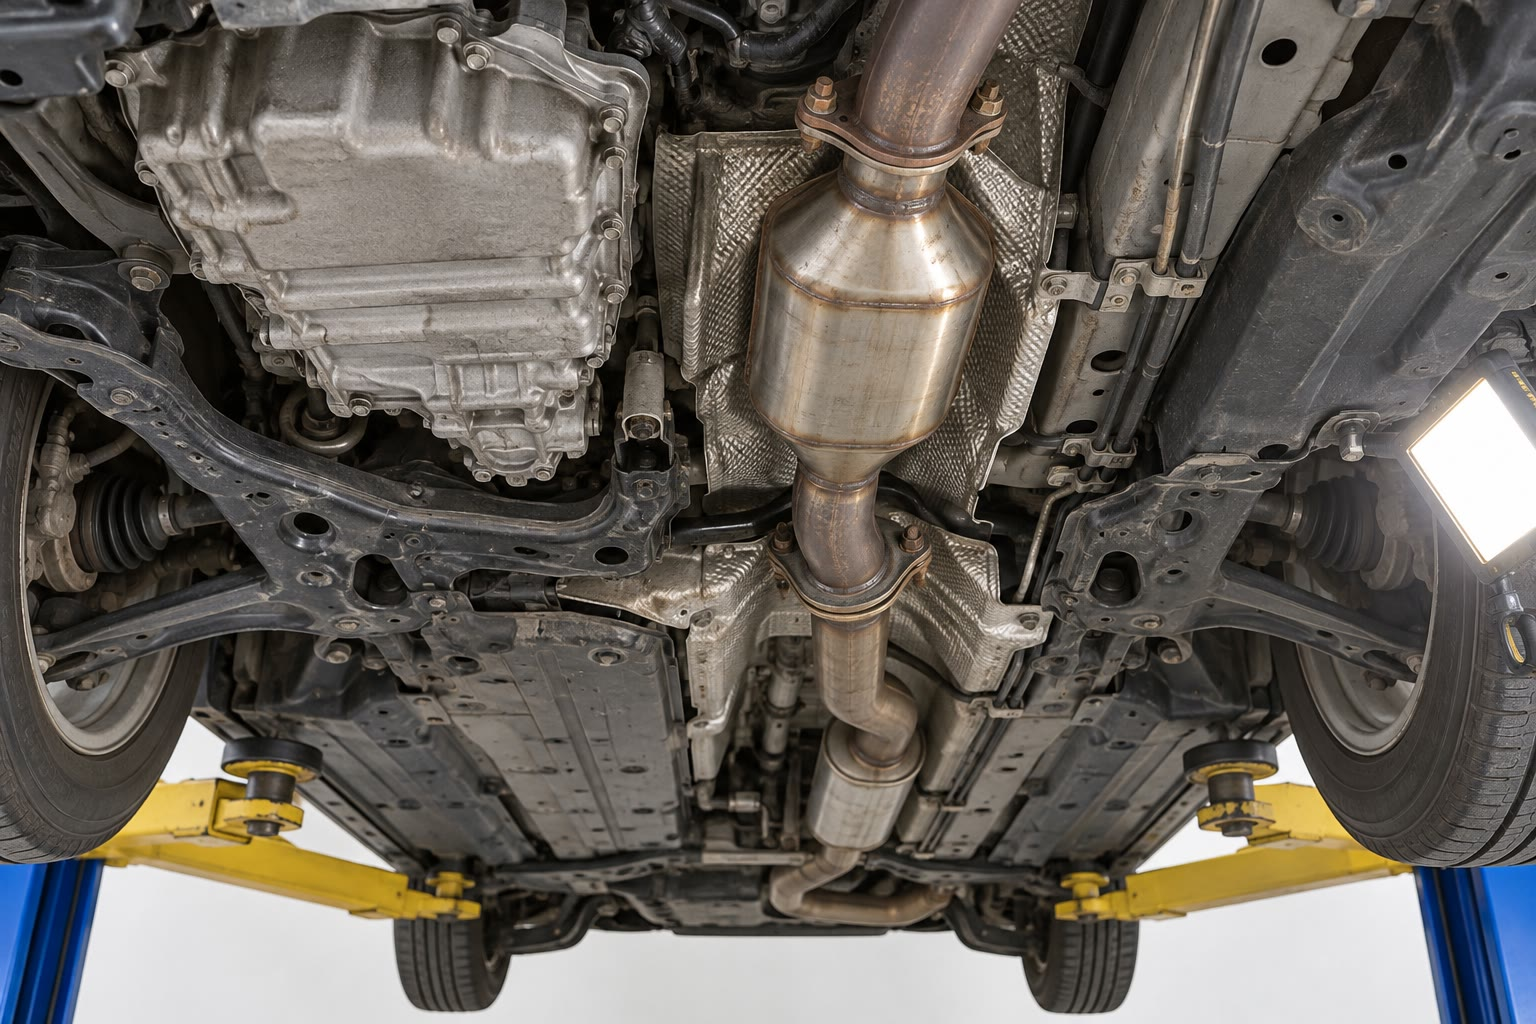
\includegraphics[width=0.5\linewidth]{images/book2/ai/b1-09-catalytic-converter.jpg}

{\small 汽车底部：排气管路中的罐体即为
催化转化器，是一种多相催化剂，
废气在其金属表面发生反应。}
\end{omfigure}

\begin{definition}[动力学控制与热力学控制]\label{def:b1:elementary-steps:control}
当一种反应物可经两条相互竞争的途径生成两种产物时，
若产物比例由生成速率决定，则反应处于\emph{动力学控制}\index{动力学控制}之下
（势垒较低的产物占优）；
若途径可逆且体系达到平衡，则反应处于
\emph{热力学控制}\index{热力学控制}之下
（较稳定的产物占优）。
\end{definition}

\begin{example}[选择产物]\label{ex:b1:elementary-steps:control}
一种反应物生成 B 的势垒为\qty{50}{kJ/mol}（$\Delta E =
\qty{-10}{kJ/mol}$），生成 C 的势垒为\qty{70}{kJ/mol}（$\Delta E =
\qty{-40}{kJ/mol}$）。在\qty{300}{K}、反应时间较短、指前因子
相等时，B 的生成速率比 C 快 $\exp(20000/(8.314 \times 300)) \approx
3000$ 倍：属动力学控制，产物为 B。在高温下，
反应时间较长时，B 可越过其较小的逆向势垒而逆转，C 则不能，
体系最终得到 C：属热力学控制。
\end{example}

\begin{history}[催化，1835 年]
1835 年，瑞典化学家约恩斯·雅各布·贝采利乌斯将十余项令人费解的观察归于一个词——
淀粉在酸的作用下变为糖，
过氧化氢被金属分解，乙醇在铂上被氧化——
并将其背后隐藏的作用力称为“催化”。直到
十九世纪末，借助奥斯特瓦尔德的动力学研究，
催化剂才被定义为：能改变反应速率、却不改变平衡的物质。
\end{history}

\section{练习}

\begin{exercise}[$\star$]\label{exo:b1:elementary-steps:1}
给出每一步的反应分子数，并说明哪些步骤可以是基元反应：
(a) $\ce{N2O5 -> NO2 + NO3}$；(b) $\ce{NO + NO3 -> 2NO2}$；
(c) $\ce{2H2 + O2 -> 2H2O}$；(d) $\ce{O + O2 + N2 -> O3 + N2}$。
\end{exercise}

\begin{exercise}[$\star$]\label{exo:b1:elementary-steps:2}
写出基元反应 $\mathrm{A} + \mathrm{B} \to
\mathrm{C}$、$2\,\mathrm{A} \to \mathrm{B}$ 和 $\mathrm{A} \to \mathrm{B} +
\mathrm{C}$ 的速率方程。为什么总反应的速率方程不能
由其化学方程式直接写出？
\end{exercise}

\begin{exercise}[$\star$]\label{exo:b1:elementary-steps:3}
在本章给出的两步能量曲线上（中间体位于
30，过渡态分别位于 70 和 55，生成物位于 $-40$，
\unit{kJ/mol}（相对于反应物），指出中间体、
过渡态和决速步。第一步是吸热还是放热？
\end{exercise}

\begin{exercise}[$\star$]\label{exo:b1:elementary-steps:4}
催化剂使某基元反应的正向速率常数增大为原来的
$10^4$ 倍。逆向速率常数增大为原来的多少倍？
平衡常数呢？达到平衡所需的时间呢？
\end{exercise}

\begin{exercise}[$\star\star$]\label{exo:b1:elementary-steps:5}
对于 $\mathrm{A} \to \mathrm{B} \to \mathrm{C}$，$k_1 =
\qty{0.10}{s^{-1}}$，$k_2 = \qty{0.30}{s^{-1}}$，求 $t_{\max}$ 以及
$\mathrm{B}$ 的最大浓度，以 $a_0$ 为单位。
\end{exercise}

\begin{exercise}[$\star\star$]\label{exo:b1:elementary-steps:6}
对于 $\mathrm{A} \underset{k_{-1}}{\overset{k_1}{\rightleftharpoons}}
\mathrm{I} \xrightarrow{k_2} \mathrm{P}$，各步均为一级反应，对中间体
$\mathrm{I}$ 应用稳态近似，证明 $v =
\frac{k_1k_2}{k_{-1} + k_2}[\mathrm{A}]$。讨论 $k_2 \gg
k_{-1}$ 和 $k_2 \ll k_{-1}$ 两种情形。
\end{exercise}

\begin{exercise}[$\star\star$]\label{exo:b1:elementary-steps:7}
碘离子催化过氧化氢的分解：
\ce{H2O2 + I- -> H2O + IO-}（慢），然后 \ce{H2O2 + IO- -> H2O + O2 + I-}
（快）。写出总反应方程式，指出催化剂和
中间体，并给出速率方程。
\end{exercise}

\begin{exercise}[$\star\star$]\label{exo:b1:elementary-steps:8}
某一步由中性分子生成碳正离子，是一个强烈的
吸热过程。利用哈蒙德假设，解释为什么能稳定碳正离子的取代基
也会加快该步反应。
\end{exercise}

\begin{exercise}[$\star\star$]\label{exo:b1:elementary-steps:9}
在\cref{ex:b1:elementary-steps:control}中，计算生成 B 与生成 C 的速率
常数之比，分别在\qty{300}{K}与\qty{600}{K}下求得，
并加以讨论。
\end{exercise}

\begin{exercise}[$\star\star\star$]\label{exo:b1:elementary-steps:10}
气体 $\mathrm{A}$ 与任一
分子 $\mathrm{M}$ 碰撞而被活化后发生分解：$\mathrm{A} + \mathrm{M} \rightleftharpoons
\mathrm{A}^* + \mathrm{M}$（$k_1$，$k_{-1}$），然后 $\mathrm{A}^* \to
\mathrm{P}$（$k_2$）。对
$\mathrm{A}^*$ 应用稳态近似，求 $v$，并证明该反应在高压下为一级，
在低压下为二级。
\end{exercise}

\begin{exercise}[$\star\star\star$]\label{exo:b1:elementary-steps:11}
证明 $[\mathrm{B}](t)$ 的表达式，即
\cref{thm:b1:elementary-steps:consecutive}中的结果，并讨论特殊情形
$k_1 = k_2 = k$，此时 $[\mathrm{B}] = a_0kt\,\eu^{-kt}$。
\end{exercise}

\begin{exercise}[$\star\star\star$]\label{exo:b1:elementary-steps:12}
总反应 $\mathrm{A} + 2\,\mathrm{B} \to \mathrm{P} +
\mathrm{C}$ 的实验速率方程为 $v =
k[\mathrm{A}][\mathrm{B}]^2/[\mathrm{C}]$。提出一个含快速预平衡的
反应机理，以解释该速率方程。
\end{exercise}

\section{周末问题：为什么一氧化氮在低温下氧化得更快}

\begin{problem}[{周末问题——一氧化氮的三级
氧化反应，经二聚体 \ce{N2O2} 的预平衡，稳态
处理，以及负的表观活化能}]
\label{pb:b1:elementary-steps:1}
对于 \ce{2NO(g) + O2(g) -> 2NO2(g)}，在
\qty{300}{K}下的初始速率测量给出（速率单位为 \unit{mol.L^{-1}.s^{-1}}）：
\begin{center}
\begin{tabular}{cccc}
\hline
实验 & $[\ce{NO}]_0$ (mol/L) & $[\ce{O2}]_0$ (mol/L) & $v_0$ \\
\hline
1 & \num{1.0e-3} & \num{1.0e-3} & \num{1.0e-5} \\
2 & \num{2.0e-3} & \num{1.0e-3} & \num{4.0e-5} \\
3 & \num{1.0e-3} & \num{2.0e-3} & \num{2.0e-5} \\
\hline
\end{tabular}
\end{center}
在\qty{400}{K}下测得的速率常数，比在
\qty{300}{K}下小为原来的十分之一。取 $R = \qty{8.314}{J/(mol.K)}$。
提出的反应机理为
\[
  \ce{2NO <=> N2O2} \ \ (k_1, k_{-1}, \text{快}), \qquad
  \ce{N2O2 + O2 -> 2NO2} \ \ (k_2, \text{慢}).
\]

\medskip
\noindent\textbf{第一部分——观测到的规律。}
\begin{enumerate}
  \item 求关于 \ce{NO} 和 \ce{O2} 的分级数。
  \item 写出速率方程，并计算 \qty{300}{K} 下的 $k$，给出其单位。
  \item 该反应能否为一步三分子基元反应？请给出理由。
  \item 由两个温度下的数据计算表观活化能。
  \item 为什么负的活化能对于一个
        基元反应是不可能的？
  \item 写出 \ce{NO} 和 \ce{O2} 的消耗速率，
        用 $v$ 表示。
\end{enumerate}

\medskip
\noindent\textbf{第二部分——前置平衡。}
\begin{enumerate}[resume]
  \item 验证两步反应相加得到总反应，并
        命名中间体。
  \item 写出每一步的反应分子数。
  \item 写出慢步的速率。
  \item 用前置平衡近似表示 $[\ce{N2O2}]$。
  \item 推导速率方程，并与实验结果比较。
  \item 用 $k_1$、$k_{-1}$ 和 $k_2$ 表示观测速率常数。
\end{enumerate}

\medskip
\noindent\textbf{第三部分——稳态。}
\begin{enumerate}[resume]
  \item 写出完整机理下的 $\dd[\ce{N2O2}]/\dd t$。
  \item 应用稳态近似，并表示 $[\ce{N2O2}]$。
  \item 推导速率方程 $v = \dfrac{k_1k_2[\ce{NO}]^2[\ce{O2}]}{k_{-1} +
        k_2[\ce{O2}]}$。
  \item 它在哪种极限下化为第二部分的结果？
  \item 在另一极限下，各级数会变为什么？
  \item 第一部分的测量结果支持哪一种极限？
\end{enumerate}

\medskip
\noindent\textbf{第四部分——表观活化能。}
每一步都遵循阿伦尼乌斯定律，活化能分别为 $E_1 =
\qty{2}{kJ/mol}$、$E_{-1} = \qty{40}{kJ/mol}$ 和 $E_2 =
\qty{15}{kJ/mol}$。
\begin{enumerate}[resume]
  \item 写出 $\ln k$，用 $k_1$、$k_{-1}$ 和
        $k_2$ 的对数表示。
  \item 推出 $E_a = E_1 - E_{-1} + E_2$。
  \item 解释：为什么基元反应的组合可以具有
        负的表观活化能？
  \item 画出能量曲线示意图：第二个过渡态
        相对于反应物 \ce{2NO + O2} 处于何处？
  \item 以此数值计算，速率在 300 与
        \qty{400}{K} 之间变化的倍数是多少？
  \item 由各步的数值计算表观活化能，并与
        第一部分比较。
\end{enumerate}
\end{problem}
